% GENERATED FROM typst/manual/sections/01_cell_measures.typ BY scripts/typ2tex.py (v1.0.0) — DO NOT EDIT.
% Edit canonical Typst under typst/ and regenerate with: python3 scripts/typ2tex.py --root . --outdir latex

\section{Cell measures and geometric comparisons}\label{manual:m3-cells}

\paragraph{Setup: cubical cell complex and five-boundary stack.}
This section instantiates the finite axis-box complex of \mainsection{main:sec:m3-cells}
with cubical boundary \mainequation{main:eq:m3-cubical-boundary} across 2D disk and
4D tesseract-to-$\pi$ enclosures and a two-square cellular fold.
Each coordinate span is a vertex or a unit interval before rational scaling, and
increasing active-axis order fixes orientation.
The closure of one filled square contains $(4,4,1)$ cells (four vertices, four edges,
and one interior cell), while the filled four-cube contains $(16,32,24,8,1)$ cells
by dimension. These fillings and their Euclidean or axial report metric in coordinate
units $u$ are explicit conditional model choices: the inherited $Q_4$ graph supplies
vertices and $H_1$ edges, and no native higher-cell admission or physical
length/area/volume is derived here.

To keep integer cell construction strictly isolated from continuum reference constants,
declare the five-boundary stack

\[
B_{\mathrm{cell}}\to B_{\mathrm{stair}}\to B_{\mathrm{fold}}\to B_{\mathrm{audit}}\to B_{\mathrm{ext}}.
\]

All integer cell selection, weight sums, staircase boundaries, integer-root enclosures,
and chain-map checks execute inside the core stages $B_{\mathrm{core}}=(B_{\mathrm{cell}},B_{\mathrm{stair}},B_{\mathrm{fold}},B_{\mathrm{audit}})$,
while Machin arctangent bounds for $\pi$ enter strictly downstream in $B_{\mathrm{ext}}$
after the finite geometry is frozen.

\paragraph{Derivation: independent measures and filled four-cube.}
For elementary axis boxes, a $d$-cell's weight is the product of its $d$ side lengths.
The interior measure adds the weights of occupied $d$-cells, counting each cell once;
a zero weight leaves the cell present in support.
The signed boundary operator cancels shared codimension-one faces while leaving them
present in the complex, and the boundary measure adds the weights of the remaining
exposed faces. An independent oracle locates those exposed faces directly from absent
top-cell neighbours.
At four-cube edge length $a=3/2$ in coordinate units $u$, literal enumeration gives

\[
V_4=\frac{81}{16}\,u^4,\qquad B_3=27\,u^3,
\]

matching the four-volume $a^4$ and exposed boundary three-measure $8a^3$.

\paragraph{Derivation: 2D circle enclosure and axial staircase.}\label{prop:m3-staircase}
Write the full-turn constant $\tau=2\pi$: a Euclidean circle of radius $r$ has
circumference $\tau r$ and disk area $(\tau/2)r^2$.
A monotone axial quarter path with coordinate displacements $r,r$ ($r>0$) has length
$2r$ when measured as the sum of axial displacements. Four quarters therefore have
exposed length $8r$ at every subdivision, retaining the fixed discrepancy $(8-\tau)r$;
increasing numerical precision does not remove this axial-metric mismatch.

Take the closed unit disk $x^2+y^2\le1$ in declared Euclidean report coordinates.
At dyadic resolution $n\in\{1,2,4,8,16,32\}$, square microcells have
side $1/n$ in $[-1,1]^2$ (equivalently unit integer cells in $[-n,n]^2$).
The outer staircase retains integer cells whose minimum corner squared radius is strictly
below $n^2$; the inner staircase retains cells whose maximum corner squared radius is at
most $n^2$. Integer inequalities fix both supports before any evaluation of $\tau$, and
the radius report is the common maximum absolute axis coordinate $r_n=1\,u$.
An independent quarter-column calculation defines upper and lower rectangle heights
$u_i=\lceil\sqrt{n^2-i^2}\rceil$ and
$\ell_i=\lfloor\sqrt{n^2-(i+1)^2}\rfloor$, $0\le i<n$.
Monotonicity of the circle graph encloses the disk area between the two rectangle sums,
and writing each ceiling as its floor plus a remainder in $[0,1]$ telescopes the floor
differences to $n$. Consequently

\begin{equation}\label{eq:m3-disk-enclosure}
A_n^-\le A_{\mathrm{disk}}\le A_n^+,\qquad A_n^+-A_n^-=\frac{4}{n^2}\sum_{i=0}^{n-1}(u_i-\ell_i)\le\frac{8}{n}.
\end{equation}

Thus $A_n^-\le\tau/2\le A_n^+$ narrows deterministically with width at
most $8/n$ (reaching $63/256$ at $n=32$), while the exposed axial boundary
remains fixed at $C_n=8\,u$ for every $n$ and falsifies $Cr=2A$ via
$C_nr_n-2A_n^+>0$ for all $n\ge4$ (unified 2D and 4D ledger in
\tabref{tab:manual-cell-boundary-fold-ledger}).

\paragraph{Derivation: 4D tesseract-to-$\pi$ enclosure and exposed 3-boundary (opened G6).}
Extend the same declared Euclidean report coordinates to the closed unit four-ball
$B^4=\{x\in[-1,1]^4:x_1^2+x_2^2+x_3^2+x_4^2\le1\}$ inside
the bounding four-cube $[-1,1]^4$, subdivided into $(2n)^4$ cubical microcells of side
$1/n$ and four-volume $1/n^4$ at dyadic levels $n\in\{1,2,4,8,16,32\}$.
Integer selection rules again act strictly inside $B_{\mathrm{core}}$ without reading
$\pi$ or $\tau$: an integer microcell in $[-n,n]^4$ belongs to the outer support when its
minimum corner squared radius is strictly below $n^2$, and to the inner support when its
maximum corner squared radius is at most $n^2$.
Let $N_{\mathrm{in}}(n)$ and $N_{\mathrm{out}}(n)$ denote the positive-orthant counts
(computed by 16-orthant sorted multinomial symmetry and cross-checked against independent
3D-column integer-root summation plus literal 4D enumeration for $n\in\{1,2,4\}$).
The exact rational four-volume inclusion enclosure is

\[
V_{4,n}^-=\frac{16N_{\mathrm{in}}(n)}{n^4}\le\frac{\pi^2}{2}\le\frac{16N_{\mathrm{out}}(n)}{n^4}=V_{4,n}^+,\qquad V_{4,n}^+-V_{4,n}^-\le\frac{64}{n}.
\]

The deterministic width bound $64/n$ follows in each orthant by indexing integer
microcells by their minimum corner $(k_1,k_2,k_3,k_4)\in\{0,\dots,n-1\}^4$
and applying the inward diagonal shift injection
$(k_1,k_2,k_3,k_4)\mapsto m=(k_1-1,k_2-1,k_3-1,k_4-1)$ on outer
orthant cells with all $k_j\ge1$ (not on the four coordinate faces $k_j=0$),
guaranteeing $\sum_{i=1}^4(m_i+1)^2=\sum_{i=1}^4k_i^2<n^2$ (hence $m$ is an
inner cell) and leaving at most $n^4-(n-1)^4\le4n^3$ boundary cells per orthant
($16\cdot4n^3/n^4=64/n$); no probability distribution or $\sigma$ is
supplied.
Because $2V_4(B^4)=\pi^2$, exact integer square roots of the finite four-cube counts
yield a pure 4D enclosure for $\pi$ strictly inside $B_{\mathrm{core}}$ with zero Machin
arctangent terms:

\[
\pi_{\mathrm{4D},n}^-:=\frac{\lfloor\sqrt{32N_{\mathrm{in}}(n)}\rfloor}{n^2}\le\pi\le\frac{\lceil\sqrt{32N_{\mathrm{out}}(n)}\rceil}{n^2}=:\pi_{\mathrm{4D},n}^+.
\]

Writing $A_{2,n}^{\pm}:=A_n^{\pm}$ for the 2D disk bounds of
\eqref{eq:m3-disk-enclosure}, for every $n\ge2$ the cross-dimensional ratio
$\pi_{\times,n}^-:=2V_{4,n}^-/A_{2,n}^+\le\pi\le2V_{4,n}^+/A_{2,n}^-=:\pi_{\times,n}^+$
likewise brackets $\pi$ without Machin input (null at $n=1$ where $A_{2,1}^-=0$,
narrowing from $[1/2,30]$ at $n=2$ to $[72561/26656,89701/24640]$ at
$n=32$).

Crucially, the exposed three-boundary of the outer 4-ball microcell staircase must be
distinguished from the exposed three-boundary of the bounding four-cube $[-1,1]^4$.
Along each of the four coordinate axes, orthogonal projection of the outer 4-ball support
onto the remaining three coordinates equals the outer 3-ball staircase support
$V_{3,n}^+=8N_{3,\mathrm{out}}(n)/n^3$, contributing two exposed 3-faces per
projected 3-column across all four axes. Hence the exact exposed 3-boundary of the outer
4-ball staircase is

\[
B_{3,\mathrm{stair},n}^+=8V_{3,n}^+=\frac{64N_{3,\mathrm{out}}(n)}{n^3}\to_{n\to\infty}\frac{32\pi}{3}\ne2\pi^2,
\]

taking exact values $64,64,51,341/8,2443/64,$ and $9179/256$ (in $u^3$)
for $n=1,2,4,8,16,32$ and verified by literal neighbour absence on $64,512,$ and
$3264$ exposed 3-faces at $n\in\{1,2,4\}$.
By contrast, the bounding four-cube $[-1,1]^4$ has constant exposed three-boundary
$B_{3,\mathrm{box}}=8\cdot2^3=64\,u^3$ at every level, which is strictly
distinct from $B_{3,\mathrm{stair},n}^+$ for all $n\ge4$.
Both boundaries falsify the Euclidean four-ball identity $B_3r=4V_4$ at every
$n\ge2$: the exposed staircase residual
$B_{3,\mathrm{stair},n}^+-4V_{4,n}^+$ remains strictly positive (reaching
$57163/4096$ at $n=32$ and converging to $32\pi/3-2\pi^2>0$), while the
box residual $B_{3,\mathrm{box}}-4V_{4,n}^+$ grows to $172443/4096$ at $n=32$.
As in 2D, this opened \texttt{G6} extension is a declared verification model only and makes no
physical continuum claim or native higher-cell admission.

\paragraph{Specialization: cellular fold chain map, projection, and anisotropy.}
The chain-map condition \mainequation{main:eq:m3-chain-map} ($B_d^LF_d=F_{d-1}B_d^K$)
is instantiated by folding two adjacent oriented unit squares
$K_2=Q_L\cup Q_R=([0,1]\times[0,1])\cup([1,2]\times[0,1])$ onto the single
unit square $L_2=Q_*=[0,1]\times[0,1]$ via $x\mapsto\min(x,2-x)$ with $y$
fixed. Active reversal along $x$ flips orientation on the right square, giving
$F_2(Q_L)=+Q_*$ and $F_2(Q_R)=-Q_*$. The complete induced integer matrices commute
with boundary identically ($B_d^LF_d-F_{d-1}B_d^K=0$ on every vertex, edge, and
2-cell): the shared vertical seam cancels ($+1-1=0$) in $\partial(Q_L+Q_R)$, the
oriented top image vanishes ($F_2(Q_L+Q_R)=0$), and $F_1(\partial(Q_L+Q_R))=0$.
Meanwhile, the unsigned input occupied area remains $2\,u^2$ (exposed boundary $6\,u$)
and the image support has area $1\,u^2$ (exposed boundary $4\,u$). Retaining both
preimage occurrences on $Q_*$ yields unsigned multiplicity two, and every source cell
retains its inner scope, identity, construction lineage, and outer image. Distinct
projected event identities cannot be merged to certify native closure.

This certifies boundary commutation for the declared fold with retained lineage; it
certifies neither occupied-area preservation nor future response. For a dynamical
reduction, the retained state must distinguish histories with different relevant next
responses: the temporal finite control exhibits the same current with different retained
pressure and different next currents, so keeping pressure resolves that collision on the
enumerated states without proving a universal reduced dynamics.
Anisotropy is checked on a $2\times1$ rectangle with fixed axis weights $(2,1)$, whose
exposed boundary is $10\,u$; swapping only its coordinates gives $8\,u$, whereas
jointly swapping the metric with the coordinates restores $10\,u$.

\paragraph{Falsification: quarantined Machin bounds, shared-$q$ controls, and execution guards.}
Downstream in $B_{\mathrm{ext}}$, rational alternating-series enclosures for
$\tau/2=\pi=16\arctan(1/5)-4\arctan(1/239)$ with $4,8,$ and $16$
terms per series separately bound numerical reference error after geometry is frozen.
They certify $C_n-\tau r_n>0$ in 2D together with
$V_{4,n}^-\le\pi^2/2\le V_{4,n}^+$,
$\pi_{\mathrm{4D},n}^-\le\pi\le\pi_{\mathrm{4D},n}^+$, and
$32\pi/3-2\pi^2>0$ in 4D.
Shared-coefficient controls in 2D ($C=2qr$, $A=qr^2\Rightarrow Cr-2A=0$)
and in 4D ($B_3=2q^2r^3$, $V_4=(q^2/2)r^4\Rightarrow B_3r-4V_4=0$)
for $q\in\{2,3,355/113,7/2\}$ all yield zero residual
identically while failing comparison against the independently computed finite measures;
a zero residual therefore cannot identify a common coefficient.

The governing contract is \texttt{contracts/scientific/CELL\_MEASURE\_SPEC.json}.
Running \texttt{python3} \texttt{manual/scripts/aod\_cell\_measures.py} \texttt{--check-data}
reproduces \texttt{manual/data/cell\_measures/cells\_geometry.json} from the declared
construction. Reversing one face incidence while retaining endpoint incidences makes
$\partial^2c\ne0$, and reversing a folded face without its induced edge map violates
\mainequation{main:eq:m3-chain-map}. The implementation executes all twelve negative
controls: incidence orientation, fold orientation, noninteger chain-map coefficients,
duplicate occupancy, dimension mismatch, native metric promotion, many-to-one projection
reconstruction, projected closure promotion, 2D refitted refinement, conflation of
$B_{3,\mathrm{stair},4}^+=51$ with $64$, fake 4D volume enclosure failing to contain
$\pi^2/2$, and 4D refitted refinement. Companion tests further mutate face counts and
metric weights and isolate evaluation constants from construction.

\subsection{Five-boundary cell-enclosure and cellular fold D.E.C. ledger}\label{manual:m3-cells:dec-staircase-fold}

Vector \texttt{RC-035} (\texttt{manual/data/boundary\_sadar/cell\_measures\_staircase\_fold\_dec.csv},
verified by \texttt{python3 -B -m manual.engine} \texttt{--sector} \texttt{boundary\_sadar}
and \texttt{aod-core} \texttt{--verify-vectors} \texttt{--check-zero-float}) binds the
unified 2D disk and 4D tesseract microcell enclosures across $n\in\{1,2,4,8,16,32\}$
together with the two-square fold chain map $B_d^LF_d=F_{d-1}B_d^K$ along
$B_{\mathrm{cell}}\to B_{\mathrm{stair}}\to B_{\mathrm{fold}}\to B_{\mathrm{audit}}\to B_{\mathrm{ext}}$.
At $n=32$, the 2D bracket narrows to $A_{32}^+-A_{32}^-=63/256$ with
$C_{32}r-2A_{32}^+=191/128>0$ ($C_n=8$), while the 4D tesseract bracket
narrows to $V_{4,32}^+-V_{4,32}^-=4285/4096$ with pure finite-4-cube bounds
$\pi_{\mathrm{4D},32}\in[3047/1024,3389/1024]$ ($[2.975586,3.309570]$),
exposed staircase 3-boundary $B_{3,\mathrm{stair},32}^+=9179/256\ne64$,
and falsifier residual $B_{3,\mathrm{stair},32}^+-4V_{4,32}^+=57163/4096>0$,
all computed without importing continuum $\pi$ from $B_{\mathrm{ext}}$.

\begin{figure}[H]
\centering
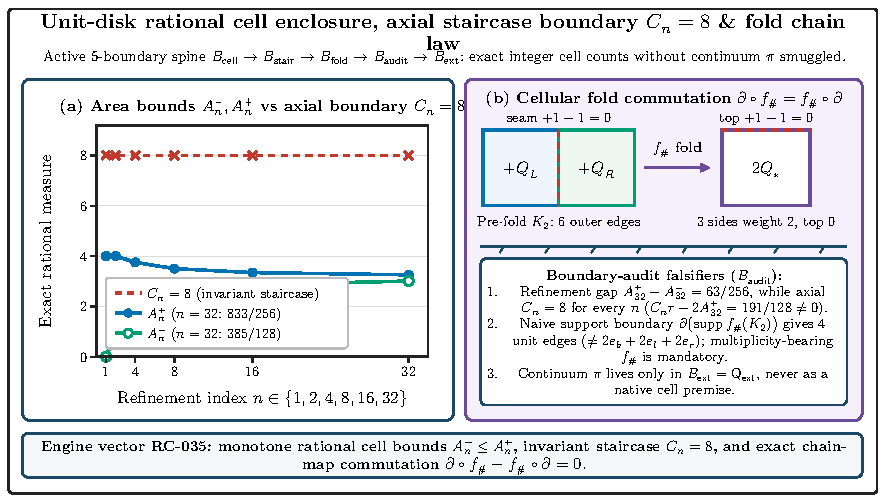
\includegraphics[width=0.92\linewidth,height=0.78\textheight,keepaspectratio]{figures/generated/cell-staircase-fold-boundary.pdf}
\caption{Projected 4D tesseract $B^4$ microcell geometry, dyadic convergence of pure 4D $\pi_{\mathrm{4D},n}^{\pm}$ and 2D $A_{2,n}^{\pm}$ bounds, 4D volume $4V_{4,n}^{\pm}\to2\pi^2$ versus exposed staircase $B_{3,\mathrm{stair},n}^+=8V_{3,n}^+\to32\pi/3$ and box $B_{3,\mathrm{box}}=64$, and two-square cellular fold commutation $B_d^LF_d=F_{d-1}B_d^K$ (\texttt{cell\_measures\_staircase\_fold\_dec.csv}).}
\label{fig:manual-cell-staircase-fold}
\end{figure}

\begin{table}[H]
\centering
\caption{Unified 2D unit-disk and opened \texttt{G6} 4D tesseract-to-$\pi$ dyadic rational enclosure and staircase falsifier ledger (\texttt{RC-035}). Throughout, $r=1\,u$, the 2D axial perimeter is fixed at $C_n=8\,u$, and the bounding 4-cube 3-boundary is fixed at $B_{3,\mathrm{box}}=64\,u^3$ (strictly distinct from $B_{3,\mathrm{stair},n}^+=8V_{3,n}^+$ for all $n\ge4$).}
\label{tab:manual-cell-boundary-fold-ledger}
{\scriptsize
\begin{tabular}{>{\raggedleft\arraybackslash}p{0.050\linewidth}>{\raggedleft\arraybackslash}p{0.067\linewidth}>{\raggedleft\arraybackslash}p{0.067\linewidth}>{\raggedleft\arraybackslash}p{0.089\linewidth}>{\raggedleft\arraybackslash}p{0.089\linewidth}>{\raggedleft\arraybackslash}p{0.089\linewidth}>{\raggedleft\arraybackslash}p{0.074\linewidth}>{\raggedleft\arraybackslash}p{0.074\linewidth}>{\raggedleft\arraybackslash}p{0.089\linewidth}>{\raggedleft\arraybackslash}p{0.128\linewidth}}
\toprule
$n$ & $A_n^-$ & $A_n^+$ & $C_nr-2A_n^+$ & $V_{4,n}^-$ & $V_{4,n}^+$ & $\pi_{\mathrm{4D},n}^-$ & $\pi_{\mathrm{4D},n}^+$ & $B_{3,\mathrm{stair},n}^+$ & $B_{3,\mathrm{stair},n}^+-4V_{4,n}^+$ \\
\midrule
1 & 0 & 4 & 0 & 0 & 16 & 0 & 6 & 64 & 0 \\
2 & 1 & 4 & 0 & 1 & 15 & $\frac{5}{4}$ & $\frac{11}{2}$ & 64 & 4 \\
4 & 2 & $\frac{15}{4}$ & $\frac{1}{2}$ & 2 & 10 & 2 & $\frac{9}{2}$ & 51 & 11 \\
8 & $\frac{41}{16}$ & $\frac{7}{2}$ & 1 & $\frac{201}{64}$ & $\frac{931}{128}$ & $\frac{5}{2}$ & $\frac{245}{64}$ & $\frac{341}{8}$ & $\frac{433}{32}$ \\
16 & $\frac{183}{64}$ & $\frac{107}{32}$ & $\frac{21}{16}$ & $\frac{8127}{2048}$ & $\frac{6201}{1024}$ & $\frac{721}{256}$ & $\frac{891}{256}$ & $\frac{2443}{64}$ & $\frac{3571}{256}$ \\
32 & $\frac{385}{128}$ & $\frac{833}{256}$ & $\frac{191}{128}$ & $\frac{72561}{16384}$ & $\frac{89701}{16384}$ & $\frac{3047}{1024}$ & $\frac{3389}{1024}$ & $\frac{9179}{256}$ & $\frac{57163}{4096}$ \\
\bottomrule
\end{tabular}
}
\end{table}
